\section{Thiết kế hệ thống}

\subsection{Kiến trúc tổng thể}
\textit{TODO: Mô tả kiến trúc client-server của hệ thống, các ứng dụng frontend, backend API và cơ sở dữ liệu PostgreSQL.}

\begin{figure}[H]
    \centering
    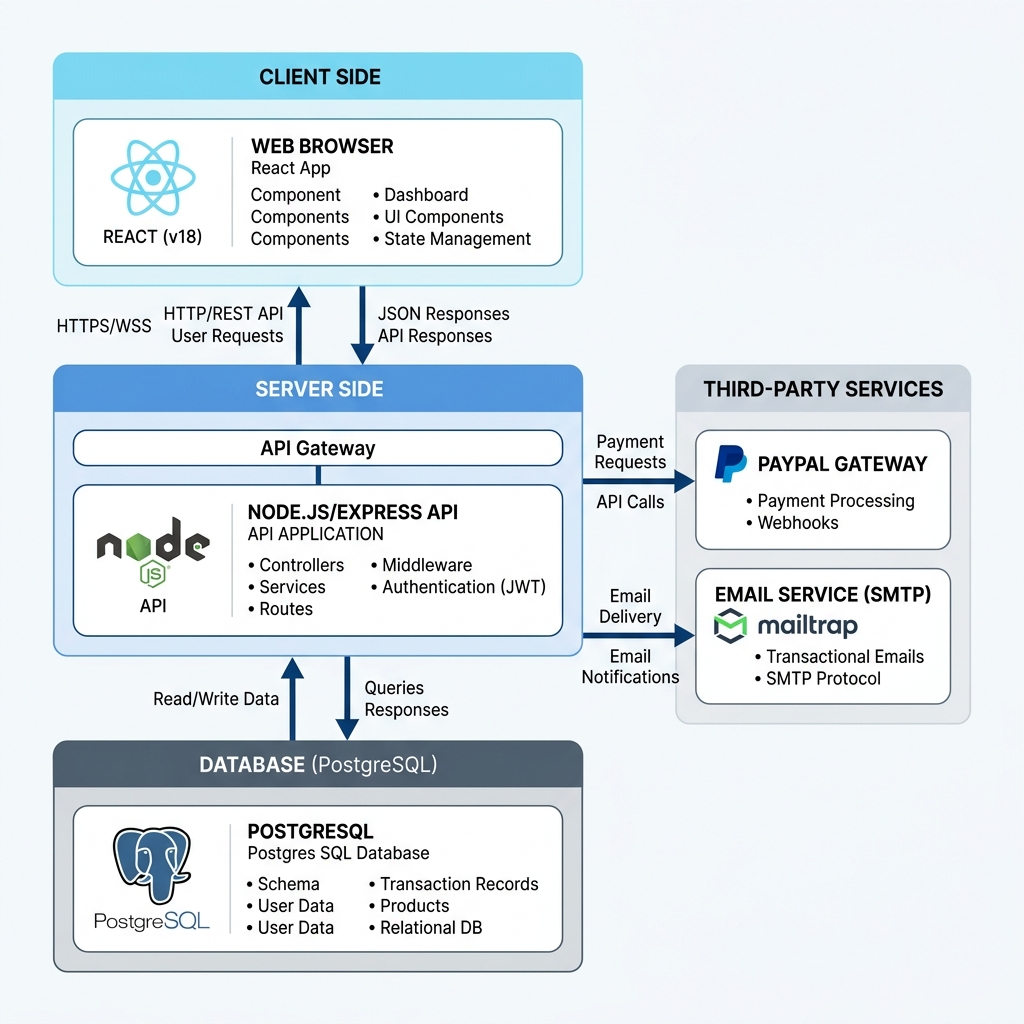
\includegraphics[width=0.85\textwidth]{images/architecture.png}
    \caption{Sơ đồ kiến trúc tổng thể hệ thống}
\end{figure}

\subsection{Các thành phần chính}
\begin{itemize}
    \item Frontend khách hàng: TODO.
    \item Frontend đối tác: TODO.
    \item Frontend quản trị: TODO.
    \item Backend API: TODO.
    \item Cơ sở dữ liệu: TODO.
    \item Dịch vụ thanh toán và gửi thông báo: TODO.
\end{itemize}

\subsection{Thiết kế luồng xử lý chính}
\textit{TODO: Mô tả các luồng nghiệp vụ quan trọng. Có thể bổ sung sequence diagram hoặc flow diagram.}

\subsubsection{Luồng đăng ký và đăng nhập}
\textit{TODO: Mô tả các bước xác thực, cấp access token, refresh token và xử lý phiên đăng nhập.}

\subsubsection{Luồng mua voucher}
\textit{TODO: Mô tả từ lúc người dùng chọn voucher, thêm vào giỏ hàng, tạo đơn hàng, thanh toán và nhận e-voucher.}

\subsubsection{Luồng sử dụng e-voucher}
\textit{TODO: Mô tả cách người dùng xem mã voucher, barcode/QR, đối tác xác nhận và cập nhật trạng thái voucher.}

\subsubsection{Luồng khiếu nại và hỗ trợ}
\textit{TODO: Mô tả cách người dùng gửi khiếu nại, hệ thống lưu thông tin và quản trị viên xử lý.}

\subsection{Thiết kế bảo mật}
\textit{TODO: Trình bày cơ chế xác thực JWT, refresh token, phân quyền API, bảo vệ thông tin người dùng và kiểm tra dữ liệu đầu vào.}

